% Author: Dominik Harmim <harmim6@gmail.com>

\documentclass[a4paper, 11pt]{scrartcl}

\usepackage[czech]{babel}
\usepackage[utf8]{inputenc}
\usepackage[T1]{fontenc}
\usepackage{times}
\usepackage[left=2cm, top=3cm, text={17cm, 24cm}]{geometry}
\usepackage[unicode, colorlinks, hypertexnames=false, citecolor=red]{hyperref}
\usepackage{fancyhdr}
\usepackage{lastpage}
\usepackage{amssymb}
\usepackage{amsmath}
\usepackage{graphicx}
\usepackage{dirtytalk}

\newcommand{\TASK}{3: Markovské řetězce a~nástroj PRISM}
\newcommand{\COURSE}{Analýza systémů založená na modelech}
\newcommand{\AUTHOR}{Dominik Harmim (xharmi00)}

\pagestyle{fancy}
\fancyhead[L]{\AUTHOR}
\fancyhead[C]{\COURSE}
\fancyhead[R]{\today}

\fancyfoot[C]{}
\fancyfoot[R]{\thepage\,/\,\pageref*{LastPage}}

\setlength{\parindent}{0pt}
\setlength{\parskip}{.5 \bigskipamount}


\begin{document}
    \begin{center}
        {\Large Úloha~\TASK}
    \end{center}


    \section*{1.~úkol}

    Zadaná \emph{reakční síť} byla namodelována v~nástroji PRISM. Výsledný
    model se nachází v~souboru \texttt{\textbf{uloha3.sm}}.

    Sémantika modelu odpovídá \emph{Markovskému řetězci ve spojitém čase
    (CTMC)}. Model obsahuje modul \texttt{cov20}, který implementuje
    danou reakční síť. Nachází se zde 3 proměnné\,---\,$ z $: počet
    \emph{zdravých} jedinců, $ n $: počet \emph{nakažených} jedinců, $ u $:
    počet \emph{uzdravených} jedinců. Každá z~těchto proměnných může nabývat
    až celkového počtu jedinců v~populaci. Iniciální hodnoty těchto
    proměnných jsou nastaveny konstantně podle zadání. Dále jsou v~modulu
    implementovány dvě reakce, které ovlivňují vývoj epidemie
    viru\,---\,\emph{nákaza}, respektive \emph{uzdravení}. Rychlosti těchto
    reakcí jsou dány parametry~$ k_i $, respektive~$ k_r $, které jsou
    definovány jako konstanty nastavované při provádění experimentů s~modelem.
    Protože model vychází z~\emph{mass-action kinetiky} pro populační modely,
    jsou rychlosti reakcí \emph{nákaza}, respektive \emph{uzdravení} nastaveny
    následovně: $ r_i = z \cdot n \cdot k_i $, respektive $ r_r = n
    \cdot k_r $.


    \section*{2.~a~3.~úkol}

    {\small \emph{Uvedené grafy jsou ve vektorovém formátu, takže je možné si
    je hezky zvětšit.}}

    Jednotlivé vlastnosti byly formulovány PCTL formulemi a~ověřeny v~nástroji
    PRISM. Tyto formule jsou specifikovány v~souboru
    \texttt{\textbf{uloha3.pctl}}.

    Vlastnost \uv{Jaká je pravděpodobnost, že infekce eventuálně vymizí?}
    byla formulována následující formulí: $ \mathrm{P}_{=?}\ [\ \mathrm{F}\ \
    n = 0\ ] $. Výsledný graf, který ukazuje odpověď na tuto otázku pro různé
    přípustné parametry~$ k_i $ a~$ k_r $ je na obrázku~\ref{fig:prop1}. Je
    zřejmé, že tato pravděpodobnost je pro všechny uvažované parametry~1.

    \begin{figure}[ht]
        \centering
        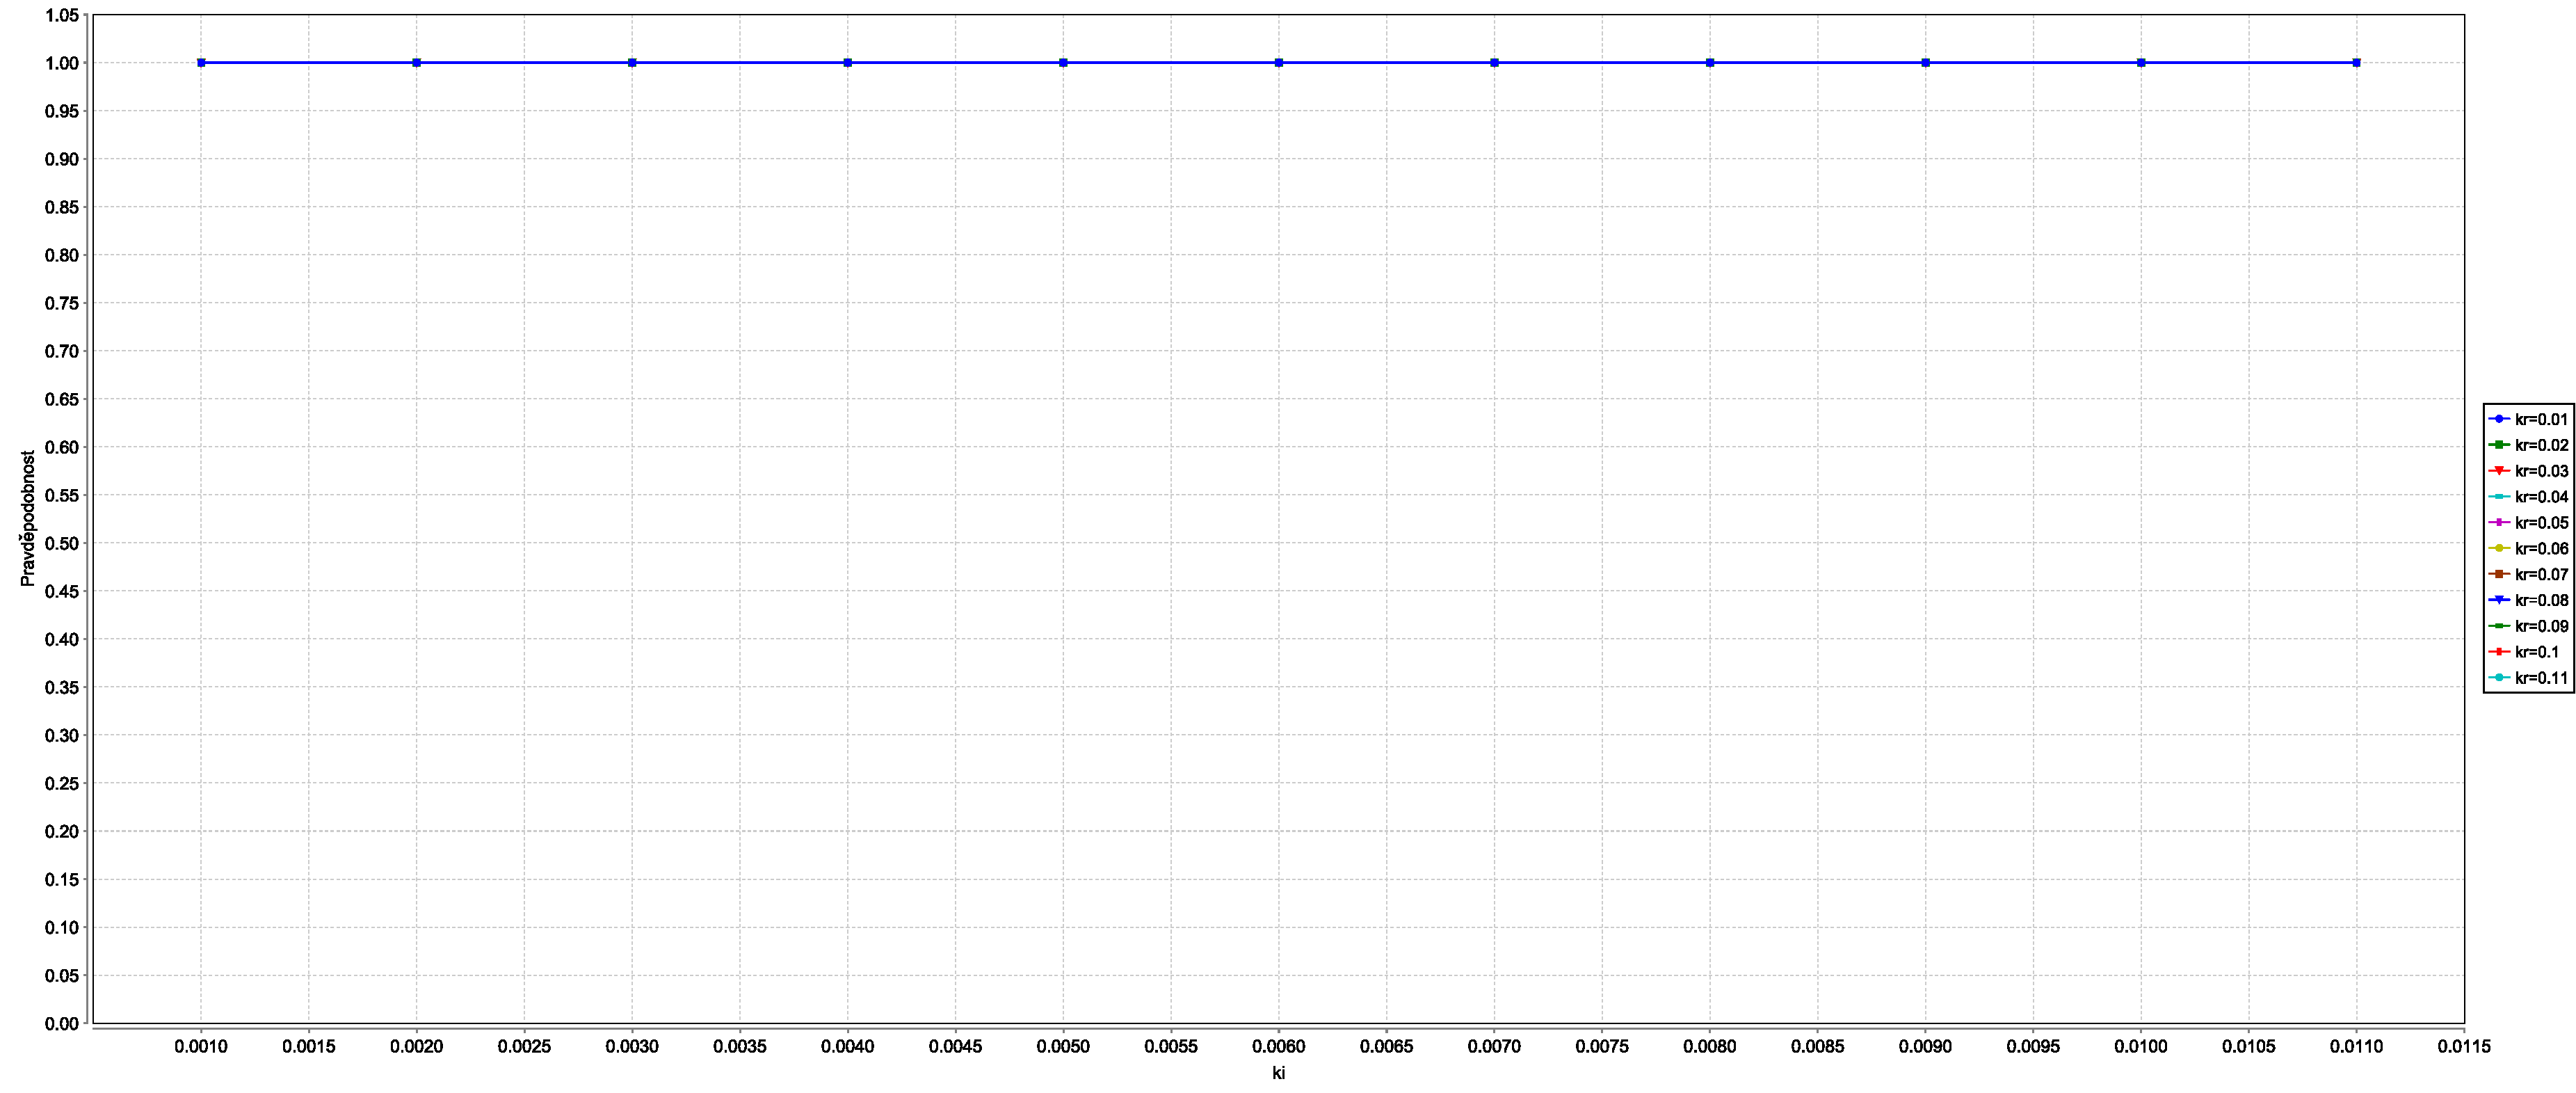
\includegraphics[width=1 \linewidth]{img/prop1.pdf}
        \caption{%
            Analýza vlastnosti \uv{Jaká je pravděpodobnost, že infekce
            eventuálně vymizí?}.
        }
        \label{fig:prop1}
    \end{figure}

    Vlastnost \uv{Jaká je pravděpodobnost, že infekce trvá aspoň 100 časových
    jednotek a~vymizí během 120 časových jednotek?} byla formulována následující
    formulí: $ \mathrm{P}_{=?}\ [\ n > 0\ \ \mathrm{U}^{[100, 120]}\ \ n = 0
    \ ] $. Výsledný graf, který ukazuje odpověď na tuto otázku pro různé
    přípustné parametry~$ k_i $ a~$ k_r $ je na obrázku~\ref{fig:prop2}.

    \begin{figure}[ht]
        \centering
        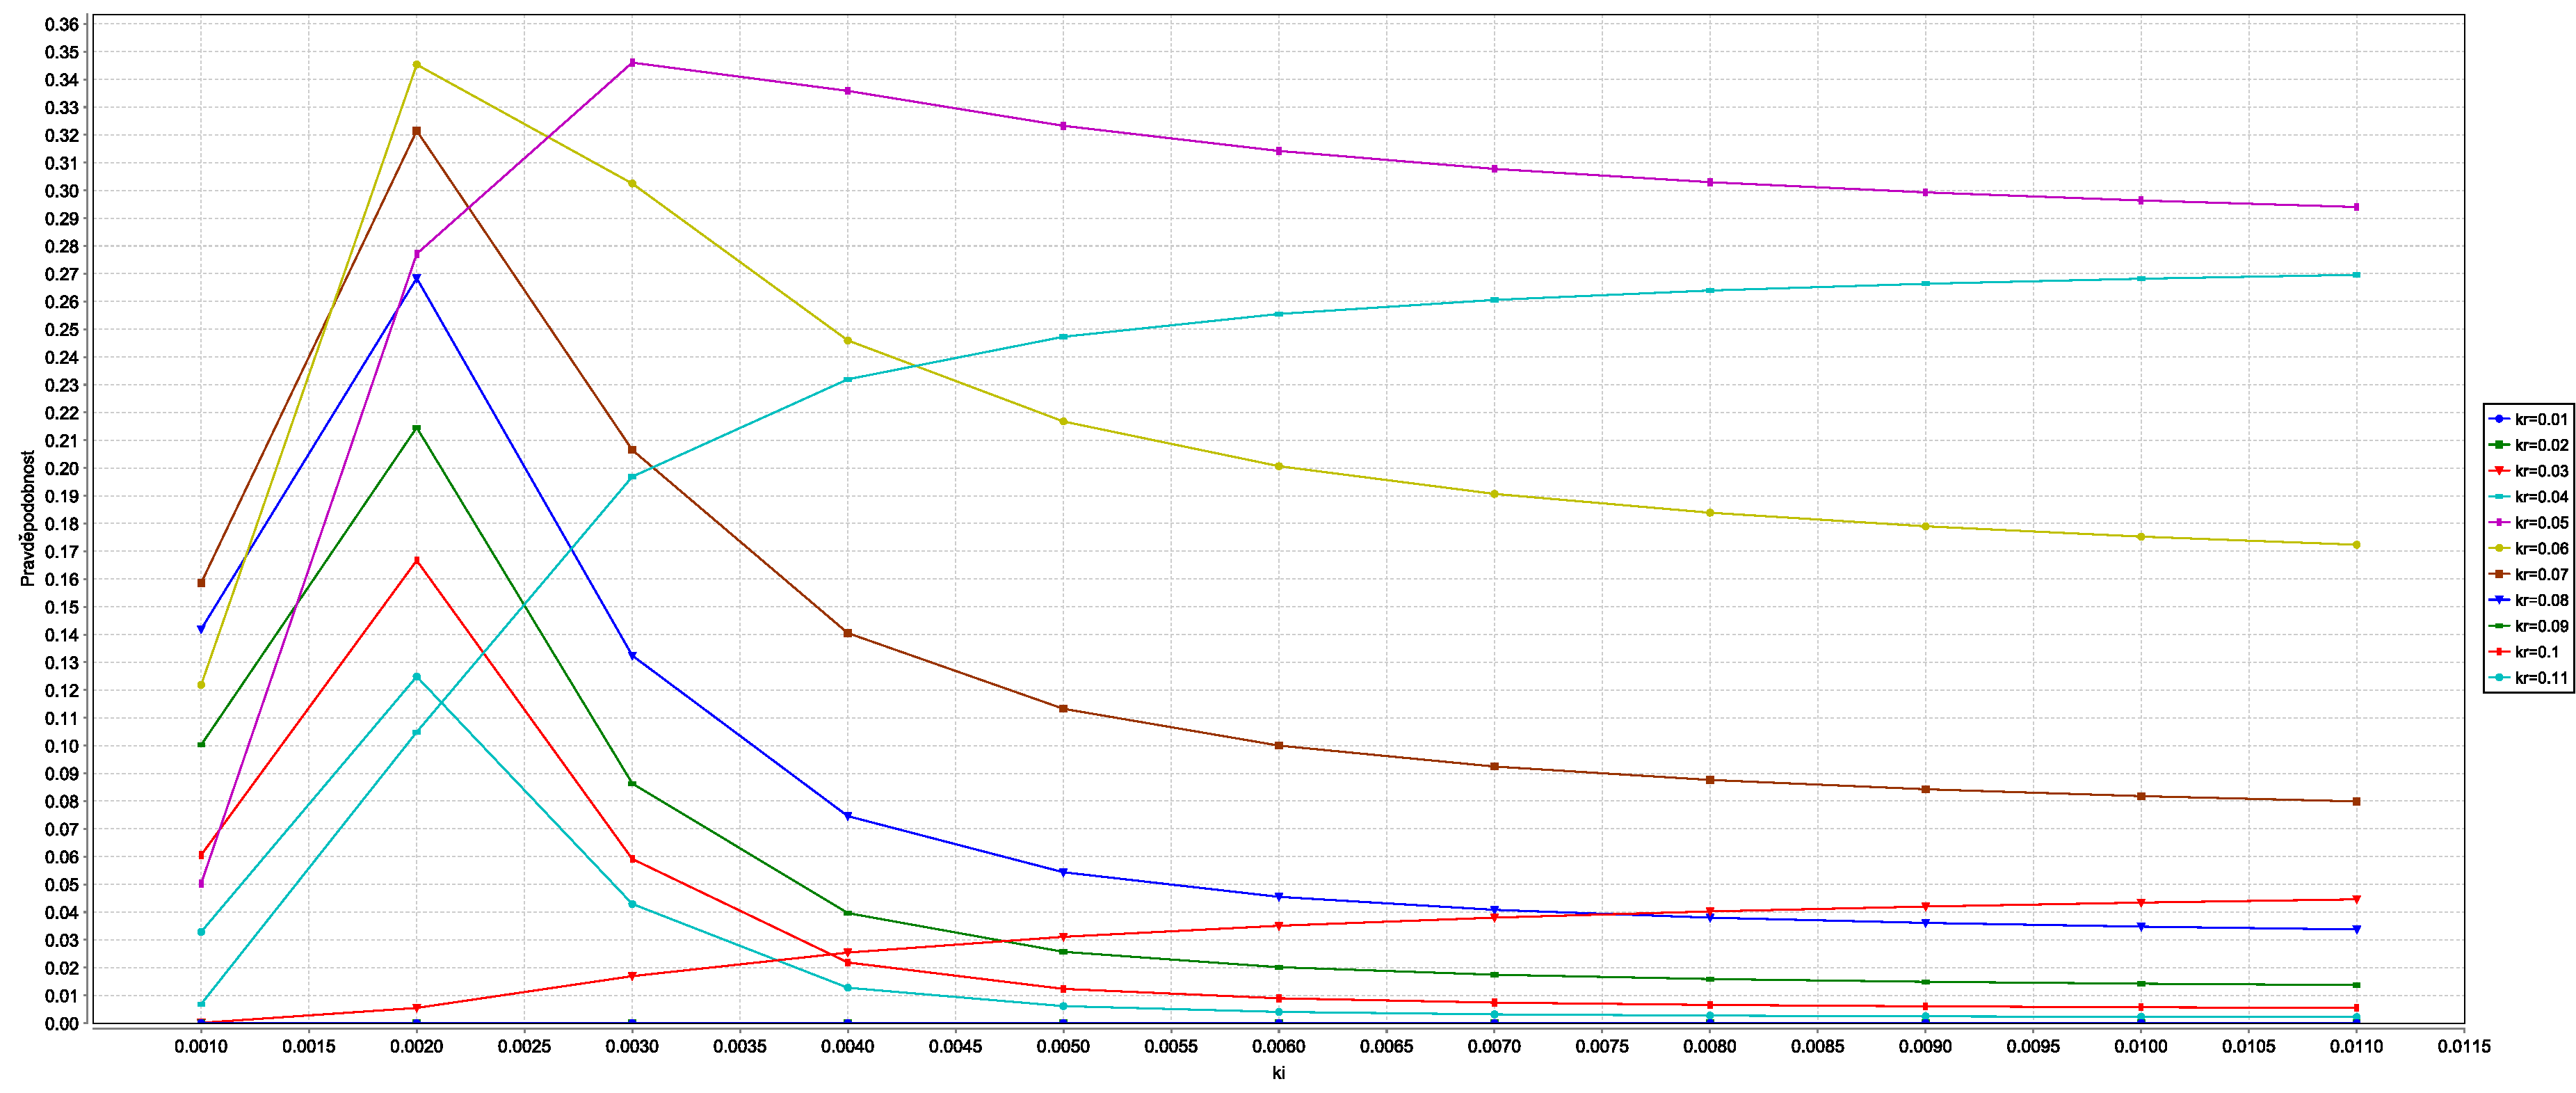
\includegraphics[width=1 \linewidth]{img/prop2.pdf}
        \caption{%
            Analýza vlastnosti \uv{Jaká je pravděpodobnost, že infekce trvá
            aspoň 100 časových jednotek a~vymizí během 120 časových jednotek?}.
        }
        \label{fig:prop2}
    \end{figure}


    \section*{4.~úkol}

    V~této nově zkonstruované reakční síti se budou vyskytovat následující
    parametry:
    \begin{itemize}
        \item
            $ k_i $: rychlost \emph{nákazy} od \emph{nakažených} jedinců
            (stejné jako v~předchozím modelu),

        \item
            $ k_j $: rychlost \emph{nákazy} od \emph{částečně vyléčených}
            jedinců (je dvakrát pomalejší, tj. $ k_j = \frac{k_i}{2} $),

        \item
            $ k_{r^\prime} $: rychlost \emph{úplného uzdravení} (stejné
            jako~$ k_r $ v~předchozím modelu s~odečtením~$ k_s $, protože
            s~rychlostí~$ k_s $ dochází místo toho k~\emph{částečnému
            uzdravení}, tj. $ k_{r^\prime} = k_r - k_s $),

        \item
            $ k_s $: rychlost \emph{částečného uzdravení} (např. $ k_s =
            \frac{k_r}{10} $).
    \end{itemize}
    Reakční síť v~této variantě bude potom vypadat následovně
    (množiny~$ Z $, $ N $, $ U $ mají stejný význam jako v~původním modelu,
    množina~$ C $ obsahuje \emph{částečně vyléčené} jedince):
    \begin{itemize}
        \item
            \emph{nákaza od nakažených jedinců}: $ Z + N \xrightarrow{k_i}
            N + N $,

        \item
            \emph{nákaza od částečně vyléčených jedinců}: $ Z + C
            \xrightarrow{k_j} N + N $,

        \item
            \emph{úplné uzdravení}: $ N \xrightarrow{k_{r^\prime}} U $,


        \item
            \emph{částečné uzdravení}: $ N \xrightarrow{k_s} C $.
    \end{itemize}
\end{document}
